
\section{Unified Framework for Feedback Analysis}
\label{sec:methodology}

This section presents our comprehensive framework for understanding, categorizing, and modeling feedback in recommender systems. We establish a unified taxonomy that enables systematic comparison across feedback types and provide rigorous analysis of algorithmic approaches.

\subsection{Multi-Dimensional Feedback Taxonomy}
\label{subsec:taxonomy}

We propose a comprehensive five-dimensional taxonomy that characterizes feedback along orthogonal axes, enabling principled analysis and optimal system design. This framework extends beyond simple implicit/explicit categorization to capture the full spectrum of feedback characteristics.

\subsubsection{Dimension 1: Collection Mechanism}
This dimension characterizes how feedback is obtained from users:

\textbf{Passive Collection}: Feedback automatically captured without user intention
\begin{itemize}
    \item \textit{Behavioral tracking}: Clicks, views, navigation patterns
    \item \textit{Physiological signals}: Eye tracking, biometric responses
    \item \textit{Environmental context}: Location, time, device characteristics
\end{itemize}

\textbf{Active Collection}: Feedback requiring deliberate user action
\begin{itemize}
    \item \textit{Direct ratings}: Numerical or categorical preference expressions
    \item \textit{Comparative judgments}: Pairwise preferences, rankings
    \item \textit{Textual feedback}: Reviews, comments, explanations
\end{itemize}

\textbf{Semi-Active Collection}: Feedback with minimal user effort
\begin{itemize}
    \item \textit{Binary indicators}: Like/dislike, thumbs up/down
    \item \textit{Implicit confirmations}: Accepting/rejecting recommendations
    \item \textit{Micro-feedback}: Quick satisfaction indicators
\end{itemize}

\subsubsection{Dimension 2: Signal Quality and Noise Characteristics}

\textbf{Signal-to-Noise Ratio}: Quantifies the reliability of preference inference
\begin{itemize}
    \item \textit{High SNR}: Direct ratings with clear semantic meaning
    \item \textit{Medium SNR}: Purchase behavior with some ambiguity
    \item \textit{Low SNR}: Click-through data with high noise levels
\end{itemize}

\textbf{Confidence Indicators}: Measures of feedback reliability
\begin{itemize}
    \item \textit{User-provided confidence}: Self-assessed certainty ratings
    \item \textit{Behavioral confidence}: Inferred from action characteristics
    \item \textit{Statistical confidence}: Derived from pattern consistency
\end{itemize}

\subsubsection{Dimension 3: Temporal Characteristics}

\textbf{Feedback Latency}: Time delay between experience and feedback
\begin{itemize}
    \item \textit{Real-time}: Immediate behavioral responses
    \item \textit{Short-term}: Feedback within hours or days
    \item \textit{Long-term}: Delayed evaluations after extended use
\end{itemize}

\textbf{Temporal Persistence}: Stability of feedback over time
\begin{itemize}
    \item \textit{Stable}: Consistent preferences across time
    \item \textit{Evolving}: Gradually changing preferences
    \item \textit{Volatile}: Rapidly fluctuating preferences
\end{itemize}

\subsubsection{Dimension 4: Cognitive Load and User Effort}

\textbf{Effort Requirements}: Cognitive and physical cost to users
\begin{itemize}
    \item \textit{Zero effort}: Automatic behavioral tracking
    \item \textit{Minimal effort}: Single-click interactions
    \item \textit{Moderate effort}: Rating scales, binary choices
    \item \textit{High effort}: Detailed reviews, explanations
\end{itemize}

\textbf{User Awareness}: Extent of user consciousness about feedback provision
\begin{itemize}
    \item \textit{Unconscious}: Automatic behavioral capture
    \item \textit{Semi-conscious}: Aware but not primary focus
    \item \textit{Conscious}: Deliberate feedback provision
\end{itemize}

\subsubsection{Dimension 5: Privacy and Sensitivity}

\textbf{Privacy Implications}: Sensitivity of feedback data
\begin{itemize}
    \item \textit{Public}: Shareable feedback (public ratings)
    \item \textit{Semi-private}: Platform-specific data (purchase history)
    \item \textit{Private}: Sensitive behavioral patterns (browsing history)
    \item \textit{Highly sensitive}: Personal/health-related preferences
\end{itemize}

\textbf{Consent Requirements}: Level of user agreement needed
\begin{itemize}
    \item \textit{Implicit consent}: Assumed through platform use
    \item \textit{Explicit consent}: Clear agreement for data collection
    \item \textit{Granular consent}: Fine-grained control over data types
\end{itemize}

\begin{figure}[ht]
\centering
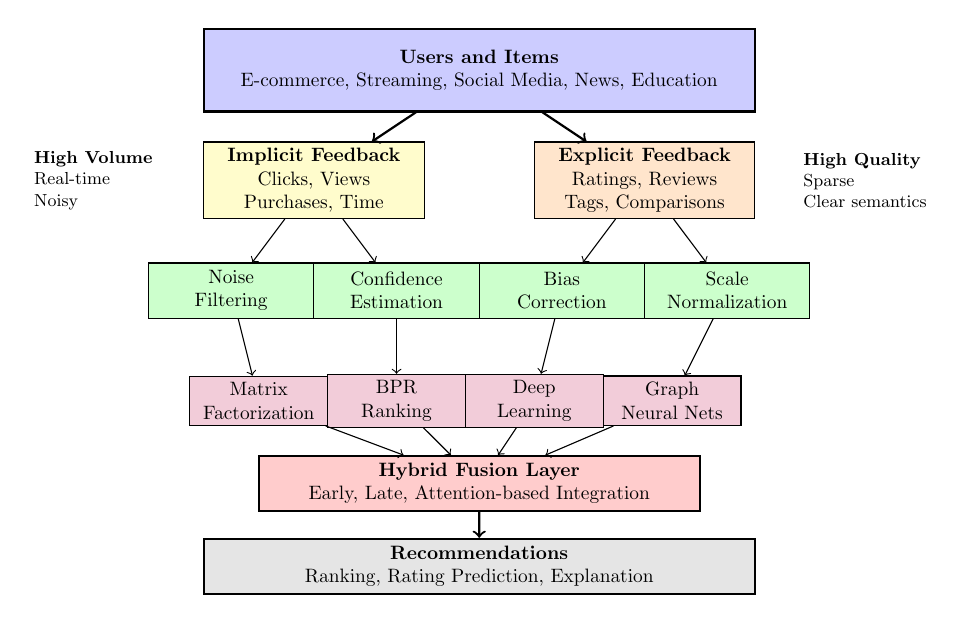
\begin{tikzpicture}[scale=0.7, transform shape]
    % User layer
    \node[rectangle, draw, thick, fill=blue!20, minimum width=10cm, minimum height=1.5cm, align=center] (users) at (0,8) {\textbf{Users and Items}\\E-commerce, Streaming, Social Media, News, Education};
    
    % Feedback collection layer
    \node[rectangle, draw, fill=yellow!20, minimum width=4cm, minimum height=1.2cm, align=center] (implicit) at (-3,6) {\textbf{Implicit Feedback}\\Clicks, Views\\Purchases, Time};
    \node[rectangle, draw, fill=orange!20, minimum width=4cm, minimum height=1.2cm, align=center] (explicit) at (3,6) {\textbf{Explicit Feedback}\\Ratings, Reviews\\Tags, Comparisons};
    
    % Processing layer
    \node[rectangle, draw, fill=green!20, minimum width=3cm, minimum height=1cm, align=center] (preprocess1) at (-4.5,4) {Noise\\Filtering};
    \node[rectangle, draw, fill=green!20, minimum width=3cm, minimum height=1cm, align=center] (preprocess2) at (-1.5,4) {Confidence\\Estimation};
    \node[rectangle, draw, fill=green!20, minimum width=3cm, minimum height=1cm, align=center] (preprocess3) at (1.5,4) {Bias\\Correction};
    \node[rectangle, draw, fill=green!20, minimum width=3cm, minimum height=1cm, align=center] (preprocess4) at (4.5,4) {Scale\\Normalization};
    
    % Algorithm layer
    \node[rectangle, draw, fill=purple!20, minimum width=2.5cm, minimum height=0.8cm, align=center] (mf) at (-4,2) {Matrix\\Factorization};
    \node[rectangle, draw, fill=purple!20, minimum width=2.5cm, minimum height=0.8cm, align=center] (bpr) at (-1.5,2) {BPR\\Ranking};
    \node[rectangle, draw, fill=purple!20, minimum width=2.5cm, minimum height=0.8cm, align=center] (deep) at (1,2) {Deep\\Learning};
    \node[rectangle, draw, fill=purple!20, minimum width=2.5cm, minimum height=0.8cm, align=center] (graph) at (3.5,2) {Graph\\Neural Nets};
    
    % Fusion layer
    \node[rectangle, draw, thick, fill=red!20, minimum width=8cm, minimum height=1cm, align=center] (fusion) at (0,0.5) {\textbf{Hybrid Fusion Layer}\\Early, Late, Attention-based Integration};
    
    % Output layer
    \node[rectangle, draw, thick, fill=gray!20, minimum width=10cm, minimum height=1cm, align=center] (output) at (0,-1) {\textbf{Recommendations}\\Ranking, Rating Prediction, Explanation};
    
    % Arrows
    \draw[thick, ->] (users) -- (implicit);
    \draw[thick, ->] (users) -- (explicit);
    \draw[->] (implicit) -- (preprocess1);
    \draw[->] (implicit) -- (preprocess2);
    \draw[->] (explicit) -- (preprocess3);
    \draw[->] (explicit) -- (preprocess4);
    \draw[->] (preprocess1) -- (mf);
    \draw[->] (preprocess2) -- (bpr);
    \draw[->] (preprocess3) -- (deep);
    \draw[->] (preprocess4) -- (graph);
    \draw[->] (mf) -- (fusion);
    \draw[->] (bpr) -- (fusion);
    \draw[->] (deep) -- (fusion);
    \draw[->] (graph) -- (fusion);
    \draw[thick, ->] (fusion) -- (output);
    
    % Side annotations
    \node[align=left, font=\small] at (-7,6) {\textbf{High Volume}\\Real-time\\Noisy};
    \node[align=left, font=\small] at (7,6) {\textbf{High Quality}\\Sparse\\Clear semantics};
    
\end{tikzpicture}
\caption{Unified System Architecture for Feedback-Aware Recommender Systems}
\label{fig:system_architecture}
\end{figure}

Figure~\ref{fig:system_architecture} presents our unified architecture that systematically processes both implicit and explicit feedback through specialized preprocessing, algorithmic modeling, and fusion components.

\subsection{Algorithmic Framework Analysis}

We systematically analyze algorithmic approaches across feedback types, organizing them into fundamental paradigms that reveal underlying principles and trade-offs.

\subsubsection{Explicit Feedback Algorithms}

\textbf{Matrix Factorization Approaches}
For explicit feedback matrix $R \in \mathbb{R}^{m \times n}$ with users $m$ and items $n$:

\begin{equation}
\min_{P,Q} \sum_{(u,i) \in \Omega} (r_{ui} - p_u^T q_i)^2 + \lambda(||P||_F^2 + ||Q||_F^2)
\end{equation}

where $P \in \mathbb{R}^{m \times k}$ and $Q \in \mathbb{R}^{n \times k}$ are user and item latent factor matrices, $\Omega$ is the set of observed ratings, and $\lambda$ is the regularization parameter.

\textbf{Neighborhood-Based Methods}
User-based collaborative filtering predicts ratings as:

\begin{equation}
\hat{r}_{ui} = \bar{r}_u + \frac{\sum_{v \in N(u)} sim(u,v) \cdot (r_{vi} - \bar{r}_v)}{\sum_{v \in N(u)} |sim(u,v)|}
\end{equation}

where $N(u)$ represents the neighborhood of user $u$, $sim(u,v)$ is user similarity, and $\bar{r}_u$ is the average rating for user $u$.

\subsubsection{Implicit Feedback Algorithms}

\textbf{Weighted Matrix Factorization}
For implicit feedback, Hu et al.~\cite{hu2008collaborative} proposed:

\begin{equation}
\min_{P,Q} \sum_{u,i} c_{ui}(p_{ui} - p_u^T q_i)^2 + \lambda(||P||_F^2 + ||Q||_F^2)
\end{equation}

where $c_{ui}$ represents confidence in the observation, $p_{ui} = 1$ if user $u$ interacted with item $i$, and $p_{ui} = 0$ otherwise.

\textbf{Bayesian Personalized Ranking}
BPR optimizes for ranking by maximizing:

\begin{equation}
\prod_{u,i,j} \sigma(\hat{r}_{ui} - \hat{r}_{uj})
\end{equation}

where $\sigma$ is the sigmoid function, and $(u,i,j)$ represents training triplets where user $u$ prefers item $i$ over item $j$.

\subsubsection{Deep Learning Approaches}

\textbf{Neural Collaborative Filtering}
NCF generalizes matrix factorization using neural networks:

\begin{equation}
\hat{r}_{ui} = f(P^T v_u^U, Q^T v_i^I | P, Q, \Theta_f)
\end{equation}

where $v_u^U$ and $v_i^I$ are one-hot encodings, $P$ and $Q$ are embedding matrices, and $\Theta_f$ represents neural network parameters.

\textbf{Autoencoder-Based Methods}
AutoRec learns user/item representations by reconstructing rating vectors:

\begin{equation}
\min_{\Theta} \sum_{u=1}^m ||r^{(u)} - f(r^{(u)}; \Theta)||_2^2 + \frac{\lambda}{2}||\Theta||_F^2
\end{equation}

where $f(\cdot; \Theta)$ is the autoencoder function with parameters $\Theta$.

\subsubsection{Hybrid Integration Strategies}

\textbf{Early Fusion}: Combine features before model training
\begin{equation}
\hat{r}_{ui} = f([x_{ui}^{impl}; x_{ui}^{expl}]; \Theta)
\end{equation}

\textbf{Late Fusion}: Combine predictions from separate models
\begin{equation}
\hat{r}_{ui} = \alpha \cdot f^{impl}(x_{ui}^{impl}) + (1-\alpha) \cdot f^{expl}(x_{ui}^{expl})
\end{equation}

\textbf{Attention-Based Fusion}: Learn dynamic combination weights
\begin{equation}
\hat{r}_{ui} = \sum_k \alpha_k \cdot f^{(k)}(x_{ui}^{(k)})
\end{equation}

where $\alpha_k = \text{softmax}(g(x_{ui}^{(k)}))$ and $g(\cdot)$ is an attention network.

\subsection{Comparative Analysis Framework}

To systematically evaluate different feedback types and algorithmic approaches, we present comprehensive comparison tables that highlight key characteristics, trade-offs, and performance considerations.

\subsubsection{Feedback Type Characteristics}
Table~\ref{tab:feedback_comparison} provides a detailed comparison of implicit and explicit feedback across multiple dimensions, enabling practitioners to make informed design decisions.

\begin{table}[ht]
\centering
\caption{Comprehensive Comparison of Feedback Types}
\label{tab:feedback_comparison}
\small
\begin{tabular}{@{}lccc@{}}
\toprule
\textbf{Characteristic} & \textbf{Implicit} & \textbf{Explicit} & \textbf{Hybrid} \\
\midrule
\multicolumn{4}{l}{\textbf{Data Collection}} \\
User Effort & None & High & Medium \\
Collection Volume & Very High & Low & High \\
Real-time Availability & Yes & No & Partial \\
Scalability & Excellent & Poor & Good \\
\midrule
\multicolumn{4}{l}{\textbf{Signal Quality}} \\
Preference Clarity & Low & High & Medium \\
Noise Level & High & Low & Medium \\
Confidence Level & Variable & High & Variable \\
Semantic Richness & Low & High & Medium \\
\midrule
\multicolumn{4}{l}{\textbf{Algorithmic Challenges}} \\
Negative Examples & Difficult & Available & Partial \\
Cold Start Problem & Severe & Moderate & Moderate \\
Sparsity Issues & Low & High & Medium \\
Computational Cost & Medium & Low & High \\
\midrule
\multicolumn{4}{l}{\textbf{System Performance}} \\
Training Speed & Fast & Medium & Slow \\
Inference Speed & Fast & Fast & Medium \\
Memory Requirements & Medium & Low & High \\
Model Complexity & Medium & Low & High \\
\midrule
\multicolumn{4}{l}{\textbf{Business Considerations}} \\
User Experience & Seamless & Intrusive & Balanced \\
Feedback Loop & Immediate & Delayed & Mixed \\
Privacy Concerns & High & Low & Medium \\
Implementation Cost & Low & Medium & High \\
\bottomrule
\end{tabular}
\end{table}

\subsubsection{Algorithmic Approach Comparison}
Table~\ref{tab:algorithm_comparison} summarizes the characteristics of major algorithmic families for different feedback types.

\begin{table}[ht]
\centering
\caption{Algorithmic Approaches by Feedback Type}
\label{tab:algorithm_comparison}
\small
\begin{tabular}{@{}lccccc@{}}
\toprule
\textbf{Algorithm} & \textbf{Implicit} & \textbf{Explicit} & \textbf{Complexity} & \textbf{Scalability} & \textbf{Performance} \\
\midrule
Neighborhood-based CF & Good & Excellent & $O(n^2)$ & Poor & Medium \\
Matrix Factorization & Excellent & Excellent & $O(nk)$ & Good & High \\
Deep Neural Networks & Excellent & Good & $O(nd)$ & Medium & High \\
BPR/Ranking Methods & Excellent & Poor & $O(n \log n)$ & Good & High \\
Graph-based Methods & Good & Good & $O(n^{1.5})$ & Medium & High \\
Autoencoder-based & Good & Excellent & $O(nd)$ & Medium & Medium \\
Attention Mechanisms & Good & Good & $O(n^2 d)$ & Poor & High \\
\midrule
\multicolumn{6}{l}{\textbf{Legend:} $n$ = users/items, $k$ = latent factors, $d$ = network depth} \\
\bottomrule
\end{tabular}
\end{table}

\begin{figure}[ht]
\centering
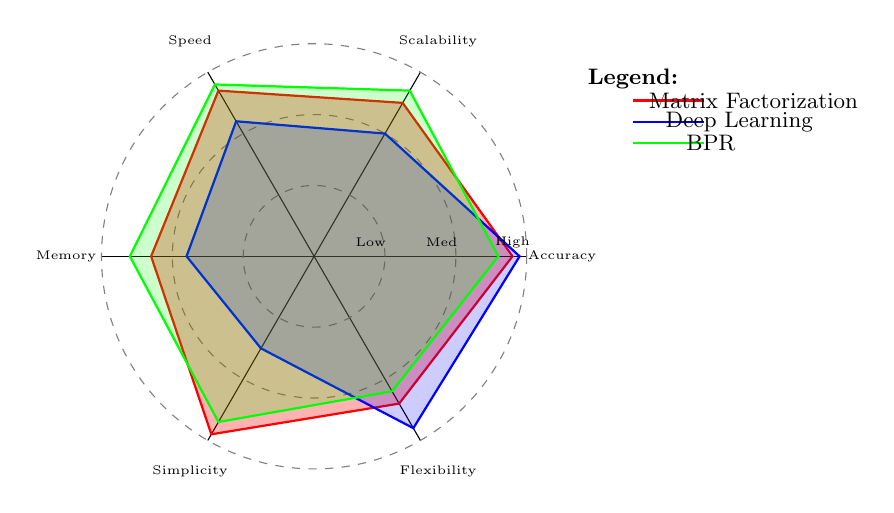
\begin{tikzpicture}[scale=0.9, transform shape]
    % Create a radar chart for algorithm comparison
    \def\n{6}
    \def\radius{3}
    
    % Draw axes
    \foreach \i in {0,...,5} {
        \draw (0,0) -- (\i*60:\radius);
        \node at (\i*60:\radius+0.5) [anchor=center] {\tiny
            \ifcase\i Accuracy\or Scalability\or Speed\or Memory\or Simplicity\or Flexibility\fi
        };
    }
    
    % Draw concentric circles
    \foreach \r in {1,2,3} {
        \draw[gray, dashed] (0,0) circle (\r);
    }
    
    % Algorithm 1: Matrix Factorization
    \coordinate (mf0) at (0*60:2.8);
    \coordinate (mf1) at (1*60:2.5);
    \coordinate (mf2) at (2*60:2.7);
    \coordinate (mf3) at (3*60:2.3);
    \coordinate (mf4) at (4*60:2.9);
    \coordinate (mf5) at (5*60:2.4);
    \draw[red, thick] (mf0) -- (mf1) -- (mf2) -- (mf3) -- (mf4) -- (mf5) -- cycle;
    \fill[red, opacity=0.3] (mf0) -- (mf1) -- (mf2) -- (mf3) -- (mf4) -- (mf5) -- cycle;
    
    % Algorithm 2: Deep Learning
    \coordinate (dl0) at (0*60:2.9);
    \coordinate (dl1) at (1*60:2.0);
    \coordinate (dl2) at (2*60:2.2);
    \coordinate (dl3) at (3*60:1.8);
    \coordinate (dl4) at (4*60:1.5);
    \coordinate (dl5) at (5*60:2.8);
    \draw[blue, thick] (dl0) -- (dl1) -- (dl2) -- (dl3) -- (dl4) -- (dl5) -- cycle;
    \fill[blue, opacity=0.2] (dl0) -- (dl1) -- (dl2) -- (dl3) -- (dl4) -- (dl5) -- cycle;
    
    % Algorithm 3: BPR
    \coordinate (bpr0) at (0*60:2.6);
    \coordinate (bpr1) at (1*60:2.7);
    \coordinate (bpr2) at (2*60:2.8);
    \coordinate (bpr3) at (3*60:2.6);
    \coordinate (bpr4) at (4*60:2.7);
    \coordinate (bpr5) at (5*60:2.2);
    \draw[green, thick] (bpr0) -- (bpr1) -- (bpr2) -- (bpr3) -- (bpr4) -- (bpr5) -- cycle;
    \fill[green, opacity=0.2] (bpr0) -- (bpr1) -- (bpr2) -- (bpr3) -- (bpr4) -- (bpr5) -- cycle;
    
    % Legend
    \node[font=\small] at (4.5,2.5) {\textbf{Legend:}};
    \draw[red, thick] (4.5,2.2) -- (5.5,2.2);
    \node[font=\small] at (6.2,2.2) {Matrix Factorization};
    \draw[blue, thick] (4.5,1.9) -- (5.5,1.9);
    \node[font=\small] at (6.0,1.9) {Deep Learning};
    \draw[green, thick] (4.5,1.6) -- (5.5,1.6);
    \node[font=\small] at (5.6,1.6) {BPR};
    
    % Scale labels
    \node[font=\tiny] at (0.8,0.2) {Low};
    \node[font=\tiny] at (1.8,0.2) {Med};
    \node[font=\tiny] at (2.8,0.2) {High};
    
\end{tikzpicture}
\caption{Algorithmic Performance Comparison Across Multiple Dimensions}
\label{fig:algorithm_performance}
\end{figure}

Figure~\ref{fig:algorithm_performance} provides a multi-dimensional comparison of major algorithmic approaches, illustrating their relative strengths and trade-offs across key performance criteria.

\subsection{Complexity Analysis and Trade-offs}

\subsubsection{Computational Complexity}
We analyze the computational requirements for different algorithmic approaches:

\textbf{Matrix Factorization}:
\begin{itemize}
    \item Training: $O(|\Omega| \cdot k \cdot t)$ where $t$ is iterations
    \item Inference: $O(k)$ per prediction
    \item Space: $O((m+n) \cdot k)$
\end{itemize}

\textbf{Deep Neural Networks}:
\begin{itemize}
    \item Training: $O(|\Omega| \cdot d \cdot t)$ where $d$ is network complexity
    \item Inference: $O(d)$ per prediction
    \item Space: $O(d)$ for parameters
\end{itemize}

\subsubsection{Feedback-Specific Considerations}

\textbf{Implicit Feedback Challenges}:
\begin{itemize}
    \item \textit{Confidence estimation}: Determining reliability of implicit signals
    \item \textit{Negative sampling}: Generating negative examples for training
    \item \textit{Temporal modeling}: Capturing evolving preferences from behavior
\end{itemize}

\textbf{Explicit Feedback Challenges}:
\begin{itemize}
    \item \textit{Sparsity handling}: Dealing with limited rating coverage
    \item \textit{Bias correction}: Addressing selection and rating biases
    \item \textit{Scale consistency}: Normalizing across different rating scales
\end{itemize}

\textbf{Hybrid System Challenges}:
\begin{itemize}
    \item \textit{Modality alignment}: Ensuring compatible representations
    \item \textit{Conflict resolution}: Handling contradictory signals
    \item \textit{Dynamic weighting}: Adapting combination strategies over time
\end{itemize}

\subsection{Theoretical Analysis and Guarantees}

\subsubsection{Convergence Properties}
We analyze convergence guarantees for different algorithmic approaches:

\textbf{Matrix Factorization}: Under appropriate regularization, alternating least squares converges to a local minimum with rate $O(1/t)$.

\textbf{BPR Optimization}: Stochastic gradient descent for BPR converges with rate $O(1/\sqrt{t})$ under standard assumptions.

\subsubsection{Generalization Bounds}
For matrix factorization with $k$ latent factors and $n$ training samples:

\begin{equation}
R(f) \leq \hat{R}(f) + O\left(\sqrt{\frac{k \log n}{n}}\right)
\end{equation}

where $R(f)$ is the true risk and $\hat{R}(f)$ is the empirical risk.

\subsection{Practical Implementation Considerations}

\subsubsection{Scalability Strategies}
\begin{itemize}
    \item \textbf{Distributed computing}: Parallelization across multiple machines
    \item \textbf{Online learning}: Incremental updates with streaming data
    \item \textbf{Approximation methods}: Randomized algorithms for large-scale systems
    \item \textbf{Caching strategies}: Efficient storage and retrieval of recommendations
\end{itemize}

\subsubsection{System Architecture Patterns}
\begin{itemize}
    \item \textbf{Lambda architecture}: Separate batch and stream processing pipelines
    \item \textbf{Microservices}: Modular services for different feedback types
    \item \textbf{Feature stores}: Centralized feature management and serving
    \item \textbf{Model serving}: Low-latency prediction infrastructure
\end{itemize}

This unified framework provides the theoretical foundation for systematic analysis of feedback mechanisms and guides the development of optimal hybrid systems that leverage the complementary strengths of different feedback types.

\paragraph{Qualitative Explicit Feedback}
\begin{itemize}
    \item \textbf{Textual reviews}: Written opinions, critiques, and detailed feedback.
    \item \textbf{Tags and categories}: User-assigned labels and classifications.
    \item \textbf{Feature ratings}: Specific aspect ratings (e.g., "sound quality: 4/5, plot: 3/5").
    \item \textbf{Comparative feedback}: Direct comparisons between items or against expectations.
\end{itemize}

\paragraph{Interactive Explicit Feedback}
\begin{itemize}
    \item \textbf{Conversational feedback}: Dialogue-based preference elicitation through chat interfaces.
    \item \textbf{Preference surveys}: Structured questionnaires and preference profiling.
    \item \textbf{Active learning queries}: System-initiated questions to clarify user preferences.
\end{itemize}

\subsection{Feedback Properties and Characteristics}

Feedback types exhibit distinct properties that influence their utility, reliability, and modeling requirements. Understanding these properties is crucial for designing appropriate algorithms and evaluation metrics.

\subsubsection{Data Abundance and Collection Dynamics}

\begin{table}[h]
\centering
\caption{Comparative Analysis of Feedback Properties}
\label{tab:feedback_properties_detailed}
\begin{tabular}{@{}lcccc@{}}
\toprule
Property & Implicit Feedback & Explicit Feedback & Hybrid Approaches & Key Implications \\
\midrule
Data Volume & Very High & Low-Moderate & High & Scalability trade-offs \\
Collection Cost & Near Zero & High (User Effort) & Variable & Economic considerations \\
Temporal Resolution & Real-time & Delayed & Mixed & Adaptation speed \\
Semantic Clarity & Low & High & Moderate & Interpretation complexity \\
Noise Level & High & Low-Moderate & Moderate & Signal processing needs \\
Sparsity Pattern & Extreme (Many zeros) & Variable & Reduced & Matrix completion challenges \\
Bias Types & Behavioral & Self-selection & Compound & Fairness requirements \\
Privacy Sensitivity & Moderate & High & High & Regulatory compliance \\
User Burden & None & High & Moderate & Engagement strategies \\
Contextual Richness & High & Low-Moderate & High & Personalization depth \\
\bottomrule
\end{tabular}
\end{table}

\subsubsection{Noise Characteristics and Signal Quality}

Implicit feedback is inherently noisy due to ambiguous user intent:
\begin{itemize}
    \item \textbf{False positives}: Clicks that don't indicate genuine interest (accidental, curiosity-driven)
    \item \textbf{Contextual noise}: Behaviors influenced by external factors (time pressure, distractions)
    \item \textbf{Platform artifacts}: Behaviors driven by UI design rather than preferences
    \item \textbf{Multi-user signals}: Shared devices or accounts introducing confounding signals
\end{itemize}

Explicit feedback, while clearer, has different noise characteristics:
\begin{itemize}
    \item \textbf{Mood-dependent bias}: Ratings influenced by temporary emotional states
    \item \textbf{Social desirability bias}: Users providing socially acceptable rather than genuine opinions
    \item \textbf{Recency bias}: Recent experiences disproportionately influencing feedback
    \item \textbf{Scale interpretation variance}: Different users interpreting rating scales differently
\end{itemize}

\subsubsection{Temporal and Contextual Dimensions}

Feedback evolves over time and varies by context:
\begin{itemize}
    \item \textbf{Short-term vs. long-term preferences}: Immediate reactions vs. stable tastes
    \item \textbf{Situational context}: Preferences varying by time of day, location, or social setting
    \item \textbf{Device-dependent behaviors}: Different interaction patterns on mobile vs. desktop
    \item \textbf{Cohort effects}: Generational differences in feedback provision and interpretation
\end{itemize}

\subsection{Advanced Feedback Categorization}

\subsubsection{Feedback Granularity Spectrum}

\begin{figure}[h]
\centering
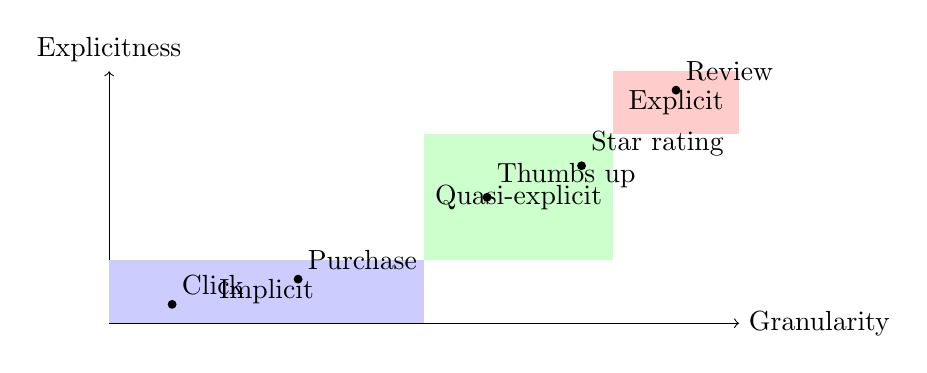
\begin{tikzpicture}[scale=0.8]
    \draw[->] (0,0) -- (10,0) node[right] {Granularity};
    \draw[->] (0,0) -- (0,4) node[above] {Explicitness};

    % Implicit region
    \fill[blue!20] (0,0) rectangle (5,1);
    \node at (2.5,0.5) {Implicit};

    % Quasi-explicit region
    \fill[green!20] (5,1) rectangle (8,3);
    \node at (6.5,2) {Quasi-explicit};

    % Explicit region
    \fill[red!20] (8,3) rectangle (10,4);
    \node at (9,3.5) {Explicit};

    % Example points
    \fill[black] (1,0.3) circle (2pt) node[above right] {Click};
    \fill[black] (3,0.7) circle (2pt) node[above right] {Purchase};
    \fill[black] (6,2) circle (2pt) node[above right] {Thumbs up};
    \fill[black] (7.5,2.5) circle (2pt) node[above right] {Star rating};
    \fill[black] (9,3.7) circle (2pt) node[above right] {Review};
\end{tikzpicture}
\caption{Feedback Granularity Spectrum}
\label{fig:granularity_spectrum}
\end{figure}

\subsubsection{Multimodal Feedback Integration}

Modern systems increasingly combine multiple feedback modalities:
\begin{itemize}
    \item \textbf{Text-visual feedback}: Product images with review text
    \item \textbf{Audio-temporal feedback}: Music listening with skip behaviors
    \item \textbf{Spatial-temporal feedback}: Location-based preferences over time
    \item \textbf{Social-contextual feedback}: Group preferences in social settings
\end{itemize}

\subsubsection{Feedback Reliability Metrics}

Different feedback types have varying reliability characteristics:
\begin{itemize}
    \item \textbf{Internal consistency}: How consistent feedback is within a user
    \item \textbf{External validity}: How well feedback predicts actual behavior
    \item \textbf{Temporal stability}: How consistent feedback is over time
    \item \textbf{Cross-platform consistency}: Feedback agreement across different contexts
\end{itemize}

\subsection{Data Collection Mechanisms and Infrastructure}

\subsubsection{Implicit Feedback Collection}

Implicit feedback collection requires sophisticated tracking infrastructure:
\begin{itemize}
    \item \textbf{Event logging systems}: Real-time capture of user interactions
    \item \textbf{Cookie and session tracking}: Maintaining user identity across sessions
    \item \textbf{Device fingerprinting}: Cross-device user identification
    \item \textbf{Third-party data integration}: Incorporating external behavioral signals
\end{itemize}

\subsubsection{Explicit Feedback Collection}

Explicit feedback requires user interface design and motivation strategies:
\begin{itemize}
    \item \textbf{Rating interfaces}: Intuitive widgets for preference expression
    \item \textbf{Incentive systems}: Gamification and rewards for feedback provision
    \item \textbf{Progressive disclosure}: Multi-step feedback collection to reduce burden
    \item \textbf{Conversational interfaces}: Natural language feedback elicitation
\end{itemize}

\subsubsection{Hybrid Collection Strategies}

Combining collection approaches for comprehensive feedback:
\begin{itemize}
    \item \textbf{Implicit-explicit cascades}: Using implicit signals to trigger explicit feedback requests
    \item \textbf{Multi-touch attribution}: Combining multiple feedback sources for robust signals
    \item \textbf{Adaptive collection}: Dynamically adjusting feedback requests based on user engagement
\end{itemize}

\subsection{Privacy and Ethical Considerations}

\subsubsection{Privacy Implications by Feedback Type}

\begin{table}[h]
\centering
\caption{Privacy and Ethical Dimensions of Feedback Types}
\label{tab:privacy_ethics}
\begin{tabular}{@{}lccc@{}}
\toprule
Dimension & Implicit Feedback & Explicit Feedback & Key Concerns \\
\midrule
Data Sensitivity & Moderate & High & Personal opinion disclosure \\
Collection Transparency & Low & High & User awareness \\
Consent Requirements & Minimal & Explicit & Legal compliance \\
Anonymization Needs & Moderate & High & Identity protection \\
Behavioral Surveillance & High & Low & Privacy erosion \\
Data Minimization & Challenging & Feasible & Storage efficiency \\
User Control & Limited & High & Autonomy preservation \\
Third-party Sharing & Common & Rare & Data brokerage risks \\
\bottomrule
\end{tabular}
\end{table}

\subsubsection{Ethical Challenges}

Feedback collection raises several ethical concerns:
\begin{itemize}
    \item \textbf{Consent and transparency}: Users often unaware of implicit data collection
    \item \textbf{Algorithmic bias amplification}: Feedback patterns reflecting societal biases
    \item \textbf{Manipulation risks}: Systems influencing user behavior through feedback incentives
    \item \textbf{Privacy-utility trade-offs}: Balancing personalization benefits with privacy costs
\end{itemize}

\subsection{Visual Taxonomy and Conceptual Framework}

Figure~\ref{fig:comprehensive_taxonomy} presents our comprehensive taxonomy of feedback types.

\begin{figure}[h]
\centering
\fbox{
\begin{minipage}{0.9\textwidth}
\textbf{Comprehensive Feedback Taxonomy}

\textbf{Main Categories:}
\begin{itemize}
\item \textbf{Implicit Feedback:} User behaviors without conscious effort
  \begin{itemize}
  \item \textit{Micro-level:} Clicks, dwell times, scrolls, hovers
  \item \textit{Meso-level:} Sessions, browsing patterns, purchase sequences
  \item \textit{Macro-level:} Longitudinal behavior, seasonal patterns, life-stage changes
  \end{itemize}
\item \textbf{Explicit Feedback:} Conscious user expressions
  \begin{itemize}
  \item \textit{Quantitative:} Ratings (1-5 stars), numerical scores, Likert scales
  \item \textit{Qualitative:} Reviews, comments, textual descriptions, tags
  \item \textit{Interactive:} Conversations, preference dialogs, custom profiles
  \end{itemize}
\item \textbf{Hybrid Approaches:} Combined implicit and explicit signals
  \begin{itemize}
  \item Multi-modal fusion, confidence-weighted integration, adaptive balancing
  \end{itemize}
\end{itemize}

\textbf{Key Properties by Category:}
\begin{tabular}{@{}lccc@{}}
\toprule
Property & Implicit & Explicit & Hybrid \\
\midrule
Data Abundance & Very High & Low & High \\
Noise Level & High & Low & Medium \\
User Effort & None & High & Medium \\
Temporal Resolution & Real-time & Delayed & Adaptive \\
Interpretability & Low & High & Medium \\
Scalability & High & Moderate & High \\
Privacy Sensitivity & High & Medium & Medium \\
Bias Susceptibility & Behavioral & Selection & Balanced \\
\bottomrule
\end{tabular}
\end{minipage}
}
\caption{Comprehensive taxonomy of implicit and explicit feedback types with hierarchical organization and key properties.}
\label{fig:comprehensive_taxonomy}
\end{figure}

\subsection{Domain-Specific Feedback Characteristics}

Different application domains exhibit unique feedback patterns and requirements:

\subsubsection{E-commerce Feedback Patterns}
\begin{itemize}
    \item High implicit feedback volume from browsing and purchasing
    \item Explicit reviews crucial for trust and explainability
    \item Strong correlation between implicit browsing and explicit purchasing decisions
\end{itemize}

\subsubsection{Entertainment Feedback Dynamics}
\begin{itemize}
    \item Implicit consumption patterns (watch time, skip rates) dominate
    \item Explicit ratings often retrospective and mood-dependent
    \item Social feedback (shares, recommendations) amplifies reach
\end{itemize}

\subsubsection{Social Media Feedback Ecology}
\begin{itemize}
    \item Implicit engagement metrics drive algorithmic ranking
    \item Explicit feedback sparse but highly influential
    \item Network effects create complex feedback cascades
\end{itemize}

This comprehensive taxonomy provides a foundation for understanding the rich landscape of feedback types in recommender systems, enabling more nuanced algorithm design and evaluation approaches.

\subsection{Modeling Approaches}
\label{subsec:modeling}

This section provides an extensive review of how implicit and explicit feedback are modeled across classical and modern approaches, including hybrid methods that integrate both types. We cover algorithmic foundations, mathematical formulations, and practical implementation considerations.

\subsection{Classical Approaches}

\subsubsection{Matrix Factorization Fundamentals}

Matrix factorization decomposes user-item interaction matrices into latent factor representations. For explicit feedback, the problem is formulated as:

\begin{equation}
\min_{P,Q} \sum_{(u,i) \in \mathcal{R}} (r_{ui} - p_u^T q_i)^2 + \lambda (\|P\|^2 + \|Q\|^2)
\label{eq:explicit_mf}
\end{equation}

where $r_{ui}$ represents explicit ratings, $p_u$ and $q_i$ are user and item latent factors, and $\lambda$ is a regularization parameter.

For implicit feedback, the formulation changes to handle binary preferences:

\begin{equation}
\min_{P,Q} \sum_{(u,i) \in \mathcal{R}^+} w_{ui} (1 - p_u^T q_i)^2 + \lambda (\|P\|^2 + \|Q\|^2)
\label{eq:implicit_mf}
\end{equation}

where $\mathcal{R}^+$ denotes observed implicit interactions and $w_{ui}$ represents confidence weights.

\subsubsection{Weighted Matrix Factorization (WMF)}

WMF addresses implicit feedback sparsity by treating unobserved interactions as negative signals with varying confidence:

\begin{equation}
\min_{P,Q} \sum_{u,i} c_{ui} (p_{ui} - p_u^T q_i)^2 + \lambda (\|P\|^2 + \|Q\|^2)
\label{eq:wmf}
\end{equation}

where $c_{ui} = \alpha r_{ui}$ for observed interactions and $c_{ui} = 1$ for unobserved ones, with $r_{ui}$ being the implicit feedback strength.

\subsubsection{Bayesian Personalized Ranking (BPR)}

BPR optimizes for ranking rather than rating prediction, using pairwise preferences:

\begin{equation}
\min_{\Theta} -\sum_{(u,i,j) \in D} \ln \sigma(\hat{r}_{ui} - \hat{r}_{uj}) + \lambda_\Theta \|\Theta\|^2
\label{eq:bpr}
\end{equation}

where $D$ contains triples $(u,i,j)$ indicating user $u$ prefers item $i$ over item $j$.

\subsection{Deep Learning Architectures}

\subsubsection{Neural Collaborative Filtering (NCF)}

NCF extends matrix factorization with neural networks:

\begin{equation}
\hat{y}_{ui} = f(p_u, q_i, p_u \odot q_i | \Theta)
\label{eq:ncf}
\end{equation}

where $f(\cdot)$ is a neural network that learns complex interaction patterns from both implicit and explicit feedback.

\subsubsection{Autoencoders for Implicit Feedback}

Denoising autoencoders reconstruct user feedback vectors:

\begin{equation}
\hat{r}_u = f_\theta(f_\phi(r_u + \epsilon))
\label{eq:autoencoder}
\end{equation}

where $\epsilon$ represents noise injection to improve generalization.

\subsubsection{Graph Neural Networks (GNNs)}

GNNs model user-item interactions as graphs:

\begin{equation}
h_u^{(l+1)} = \sigma\left(\sum_{v \in \mathcal{N}(u)} \frac{1}{\sqrt{|\mathcal{N}(u)||\mathcal{N}(v)|}} W^{(l)} h_v^{(l)}\right)
\label{eq:gnn}
\end{equation}

where $\mathcal{N}(u)$ denotes neighbors in the user-item interaction graph.

\subsection{Reinforcement Learning Approaches}

\subsubsection{Markov Decision Processes for Recommendations}

Recommendations are framed as sequential decision-making:

\begin{equation}
\pi^*(s) = \arg\max_\pi \mathbb{E}\left[\sum_{t=0}^\infty \gamma^t r(s_t, a_t) \bigg| s_0 = s, \pi\right]
\label{eq:rl_mdp}
\end{equation}

where states $s$ include user context, actions $a$ are item recommendations, and rewards $r$ come from implicit feedback.

\subsubsection{Contextual Bandits}

Multi-armed bandit approaches balance exploration and exploitation:

\begin{equation}
\mu_{t+1} = \mu_t + \alpha_t (r_t - \mu_t)
\label{eq:bandit_update}
\end{equation}

where $\mu_t$ tracks expected rewards from implicit user responses.

\subsection{Contrastive Learning Paradigms}

\subsubsection{SimCLR for Recommendations}

Contrastive learning maximizes agreement between different views of user-item interactions:

\begin{equation}
\mathcal{L} = -\log \frac{\exp(\text{sim}(z_i, z_j)/\tau)}{\sum_{k=1}^{2N} \mathbb{I}_{[k \neq i]} \exp(\text{sim}(z_i, z_k)/\tau)}
\label{eq:contrastive}
\end{equation}

where $z_i, z_j$ are representations from positive pairs and $\tau$ is temperature.

\subsubsection{Hybrid Contrastive Objectives}

Combining supervised and self-supervised learning:

\begin{equation}
\mathcal{L}_{hybrid} = \mathcal{L}_{supervised} + \lambda \mathcal{L}_{contrastive}
\label{eq:hybrid_contrastive}
\end{equation}

balancing explicit supervision with implicit structure learning.

\subsection{Modern Approaches}

\subsubsection{Deep Learning Models}
Neural networks have revolutionized RS modeling. Autoencoders handle implicit feedback sparsity through reconstruction \cite{sedhain2015autorec}. Convolutional Neural Networks (CNNs) process sequential behaviors \cite{tang2018personalized}. Graph Neural Networks (GNNs) model user-item interactions as graphs \cite{wang2019neural}.

\subsubsection{Reinforcement Learning}
Reinforcement Learning (RL) frames recommendations as sequential decision-making. Implicit feedback serves as rewards, with exploration-exploitation trade-offs \cite{zhao2018recommendations}. Explicit feedback can provide more precise reward signals \cite{chen2019large}.

\subsubsection{Contrastive Learning}
Self-supervised contrastive learning leverages implicit feedback for representation learning. Methods like SimCLR adapt to RS by contrasting user-item interactions \cite{wu2021self}. Hybrid approaches combine contrastive objectives with explicit supervision \cite{xie2022contrastive}.

\subsection{Implicit-to-Explicit Conversions}

Several techniques convert implicit feedback to pseudo-explicit ratings:
\begin{itemize}
    \item \textbf{Ordinal regression}: Maps implicit signals to rating scales \cite{weston2011wsabie}.
    \item \textbf{Confidence weighting}: Assigns confidence scores to implicit preferences \cite{he2016fast}.
    \item \textbf{Generative models}: Uses GANs to synthesize explicit feedback from implicit data \cite{wang2017irgan}.
\end{itemize}

\subsection{Hybrid Models}

Hybrid approaches jointly model both feedback types:
\begin{itemize}
    \item \textbf{Multi-task learning}: Optimizes separate objectives for implicit and explicit feedback \cite{ma2011learning}.
    \item \textbf{Unified frameworks}: Integrates feedback types in shared latent spaces \cite{lian2017cccfnet}.
    \item \textbf{Attention mechanisms}: Weights different feedback sources dynamically \cite{chen2017attentive}.
\end{itemize}

\subsection{Detailed Modeling Techniques}

\subsubsection{Neural Matrix Factorization}

Neural extensions of matrix factorization use multi-layer perceptrons to model non-linear interactions. For implicit feedback, models like NeuMF \cite{he2017neural} learn from binary preferences, achieving state-of-the-art performance on ranking tasks.

\subsubsection{Sequence Modeling}

Recurrent Neural Networks (RNNs) and Transformers capture temporal dependencies in implicit feedback sequences. Models like BERT4Rec \cite{sun2019bert4rec} treat recommendation as a sequence prediction problem.

\subsubsection{Graph-Based Approaches}

Graph Neural Networks model user-item interactions as heterogeneous graphs. Methods like LightGCN \cite{he2020lightgcn} propagate preferences through graph convolutions, effectively handling implicit feedback sparsity.

\subsubsection{Generative Models}

Variational Autoencoders (VAEs) and Generative Adversarial Networks (GANs) generate synthetic feedback. For implicit data, VAEs learn latent representations that reconstruct user behavior patterns.

\subsection{Hybrid Integration Strategies}

\subsubsection{Attention-Based Fusion}

Attention mechanisms dynamically weight feedback sources. For example, in a music recommender, recent explicit ratings might receive higher attention than older implicit plays.

\subsubsection{Multi-Modal Learning}

Combining feedback with content features (e.g., item descriptions) enhances modeling. Vision-language models process explicit reviews alongside implicit clicks.

\subsubsection{Cross-Feedback Translation}

Techniques translate between feedback types. For instance, using LLMs to generate explicit ratings from implicit patterns.

\subsection{Computational Complexity and Scalability}

Implicit feedback models must handle large-scale data. Techniques like negative sampling and distributed training enable scalability. Explicit feedback models are computationally lighter but data-scarce.

\subsection{Evaluation of Modeling Approaches}

Empirical studies show that hybrid models outperform single-type approaches. However, performance gains depend on domain and data quality.

\subsection{Case Studies}

\subsubsection{YouTube Recommendations}

YouTube uses implicit watch time extensively, combined with explicit likes/dislikes. Their system employs deep neural networks for real-time personalization.

\subsubsection{Amazon Product Recommendations}

Amazon integrates purchase history (implicit) with reviews (explicit) using collaborative filtering and content-based methods.

\subsection{Advanced Implementation Considerations}

\subsubsection{Hyperparameter Optimization Strategies}

Effective hyperparameter tuning is crucial for model performance:

\begin{itemize}
    \item \textbf{Grid Search vs. Random Search}: Random search often more efficient for high-dimensional spaces
    \item \textbf{Bayesian Optimization}: Gaussian processes for sample-efficient optimization
    \item \textbf{AutoML Approaches}: Automated machine learning for hyperparameter discovery
    \item \textbf{Domain-Specific Tuning}: Different optimal parameters for implicit vs. explicit feedback
\end{itemize}

\subsubsection{Model Interpretability and Explainability}

Understanding model decisions is increasingly important:

\begin{itemize}
    \item \textbf{Attention Visualization}: Interpreting which feedback sources influence predictions
    \item \textbf{Feature Importance}: Identifying key implicit signals and explicit features
    \item \textbf{Counterfactual Explanations}: Explaining recommendations through "what-if" scenarios
    \item \textbf{User-Centric Explanations}: Translating technical model outputs to user-understandable insights
\end{itemize}

\subsubsection{Online Learning and Adaptation}

Systems must adapt to evolving user preferences:

\begin{itemize}
    \item \textbf{Incremental Learning}: Updating models with new feedback without full retraining
    \item \textbf{Concept Drift Detection}: Identifying when user preferences change significantly
    \item \textbf{Temporal Regularization}: Balancing historical and recent feedback appropriately
    \item \textbf{Context-Aware Updates}: Adapting to changing situational contexts
\end{itemize}

\subsubsection{Computational Resource Management}

Efficient deployment requires careful resource allocation:

\begin{itemize}
    \item \textbf{Model Compression}: Reducing model size for edge deployment
    \item \textbf{Inference Optimization}: Fast prediction serving for real-time recommendations
    \item \textbf{Caching Strategies}: Intelligent caching of user representations and item embeddings
    \item \textbf{Distributed Serving}: Scaling recommendation serving across multiple machines
\end{itemize}

\subsection{Emerging Algorithmic Paradigms}

\subsubsection{Multimodal Recommender Systems}

Integrating multiple data modalities for richer recommendations:

\begin{itemize}
    \item \textbf{Vision-Language Models}: Processing product images with textual reviews
    \item \textbf{Audio-Textual Integration}: Combining music audio features with user listening history
    \item \textbf{Cross-Modal Translation}: Converting between different feedback modalities
    \item \textbf{Multimodal Fusion Architectures}: Attention-based fusion of heterogeneous signals
\end{itemize}

\subsubsection{Causal Inference in Recommendations}

Understanding causal relationships rather than mere correlations:

\begin{itemize}
    \item \textbf{Causal Graphs}: Modeling causal pathways from feedback to user satisfaction
    \item \textbf{Intervention Analysis}: Simulating the effects of different recommendation strategies
    \item \textbf{Counterfactual Reasoning}: Estimating what would have happened under different conditions
    \item \textbf{Bias Mitigation}: Removing spurious correlations through causal methods
\end{itemize}

\subsubsection{Federated and Privacy-Preserving Learning}

Collaborative learning without compromising privacy:

\begin{itemize}
    \item \textbf{Federated Matrix Factorization}: Distributed training across user devices
    \item \textbf{Differential Privacy}: Adding noise to protect individual feedback
    \item \textbf{Secure Multi-Party Computation}: Privacy-preserving collaborative filtering
    \item \textbf{Homomorphic Encryption}: Encrypted computation on sensitive feedback data
\end{itemize}

\subsubsection{Continual and Lifelong Learning}

Adapting to evolving user preferences over time:

\begin{itemize}
    \item \textbf{Catastrophic Forgetting Prevention}: Maintaining old knowledge while learning new patterns
    \item \textbf{Elastic Weight Consolidation}: Protecting important parameters during updates
    \item \textbf{Progressive Neural Networks}: Growing network capacity for new tasks
    \item \textbf{Memory Replay}: Rehearsing past experiences to maintain performance
\end{itemize}

\subsection{Open Challenges in Modeling}

\begin{itemize}
    \item Handling feedback conflicts (e.g., clicking but not purchasing).
    \item Modeling long-term vs. short-term preferences.
    \item Incorporating user context and demographics.
\end{itemize}
